\chapter{Results on means and tools for primary toolchain}
\label{sec:results}

\section{Proposed Toolchains}

This chapter describes the proposed toolchains and the selection process for finding them.

There were three toolchain proposals in total (Figure~\ref{fig:proposals}).  These are:

 \begin{figure}[b!]
  \centering
  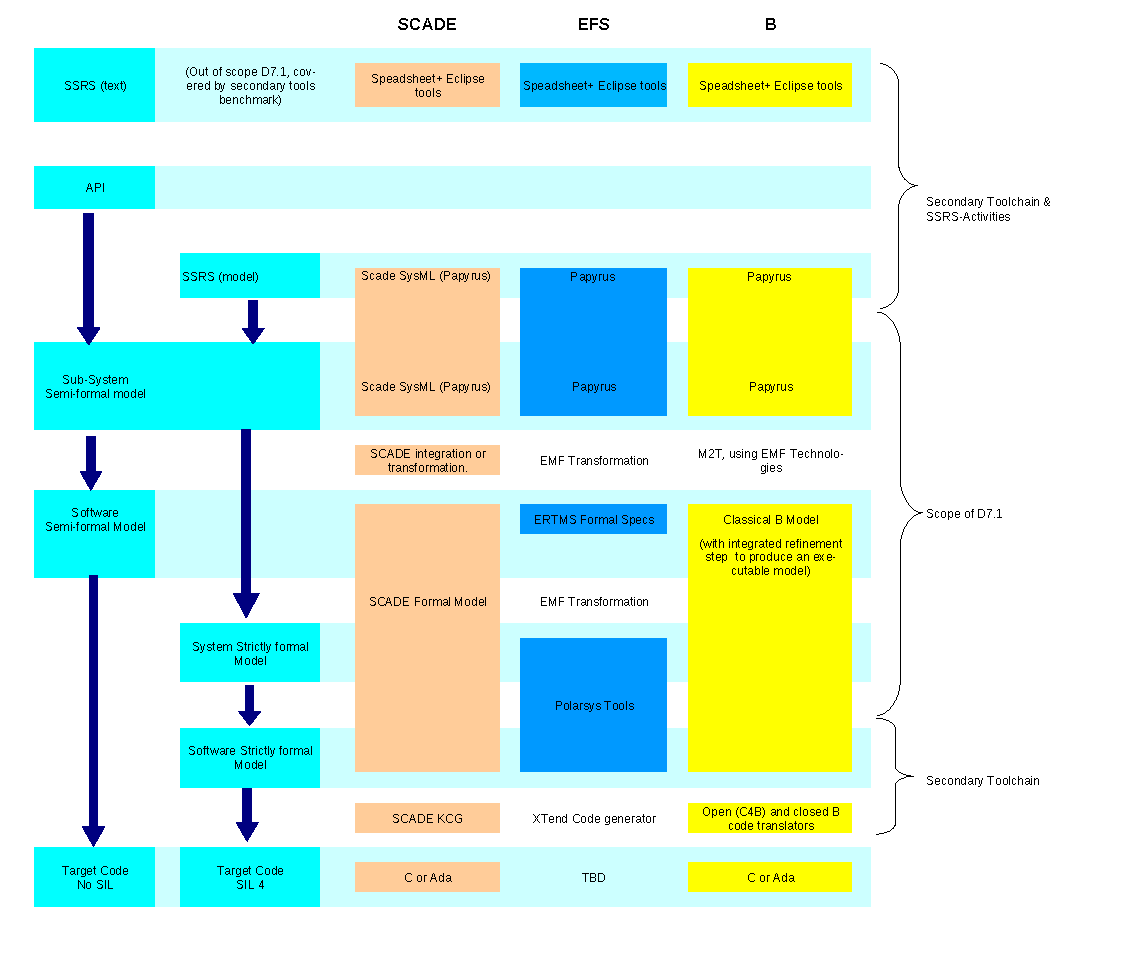
\includegraphics[width=\linewidth]{images/compare-toolchains.pdf}
  \caption{Proposed Toolchains}
  \label{fig:proposals}
\end{figure}

\begin{description}

\item[SCADE.] A SCADE-based primary toolchain would consist of the two tools Papyrus and SCADE.  An integration between the tools already exists, and both tools cover all activities.  Specifically, the SysML model can be edited with both, Papyrus and SCADE interchangeably.  The biggest advantage is that there would be little additional work necessary to cover the primary toolchain.  The biggest drawback of this solution is the fact that SCADE is not open source.  However, its artefacts (SysML, XML, Lystre, ASCII text, PDF, C or ADA) are openly defined and can therefore be incorporated into open documents, models, or software.
At the lowest level, the code generation, other alternative code generators could be used as well. Within the scope of the openETCS project no development work is planned to adapt SCADE tools to the open proofs tools chain, as long as SCADE is not licensed under an OSI certified open source license.

\item[ERTMS Formal Specs (EFS).] An EFS-based primary toolchain would mainly consist of the EFS tool itself and optional with additional components from the Eclipse ecosystem, looking at Polarsys for guidance. This toolchain is mainly intended to support the semi-formal modeling and non vital code (no SIL) generation process. (For verification purposes of functional correctness, a second model could be used in parallel.)
The biggest advantage of this approach is that it is open source, and that a significant portion of Subset 26 has already modeled with EFS, since it can already be ``used as is''. The biggest drawback is that EFS is only partly ported to Eclipse, and that it is not clear how laborious the tailoring of the Eclipse-based code generator would be or if any Eclipse-based code generators could be adapted to accommodate these functions. During the course of the project issues are supposed to be collected in order to continuously improve the EFS toolchain and integrate it into Eclipse.

%An EFS-based primary toolchain would mainly consist of the Papyrus, EFS and additional components from the Eclipse ecosystem, looking at Polarsys for guidance.  It is not clear if and how the formal models could be modeled with this toolchain.  The biggest advantage of this approach is that it is open source, and that a significant portion of Subset 26 has already modeled with EFS.  The biggest drawback is that it is not clear how the integration with Papyrus would look like, that EFS is only partly ported to Eclipse, and that it is not clear how laborious the tailoring of the Eclipse-based formal modeling tools would be.

\item[B.] In contrast to the previous proposals, this one starts bottom-up, starting with the assumption that code generation from B models is possible and practical.   This toolchain proposes working with B on the bottom two layers, but leaves open how these are connected to the Papyrus-based top.  The biggest advantage of this approach is that the resulting model will be usable, and that there is a rich existing ecosystem for B, both open source and commercial.  The biggest drawback is that there are many blanks to fill in, which may require significant development work.

\end{description}

\section{Selection Process}

The selection process consisted of the six steps shown here, with more detail being provided below.

\begin{description}

\item[Benchmarking. (Section~\ref{sec:benchmarking})] Project partners were asked to step up and perform a benchmark of the tool of their choice.  The proposals were checked against D2.1 (State of the art) to make sure that no important tools were missed (or if so, why).  Not all benchmarks were completed, CORE, Why3 and UPPAAL dropped out.  Further, after completing the benchmark, GOPPR, GNATprove and Petri Nets were dropped due to the evaluation results.

\item[Assessment (Section~\ref{sec:assessment}).] Each Benchmark was assessed by its author and by two additional assessors (in the case of Petri Nets and GNATprove, there was just one assessor).  The assessment quantified evaluation criteria, resulted in a report consisting of hundreds of scores for each completed benchmark.

\item[Decision Meeting (Section~\ref{sec:decision_meeting}).] A decision meeting took place to eliminate tools and to start looking at possible tool configuration that would form the primary toolchain.  During this meeting, Enterprise Architect (SysML) was also eliminated, in favor of the open source alternative Papyrus.  Papyrus/SCADE was identified as one promising toolchain.  Last, Papyrus had been selected as the tool for the Sub System Semi-formal model.

\item[Composition of Toolchains (Section~\ref{sec:composition_of_tool_chains}).] With the number of tools reduced significantly and one selected tool (Papyrus), team members were invited to propose concrete toolchains covering the primary toolchain.  This resulted in two more proposals, in addition to Papyrus/SCADE.

\item[Documenting the Decision (Section~\ref{sec:documenting_the_decision}).] This deliverable documents the three toolchains, as well as their respective strengths and weaknesses.  As has been determined a long time ago\footnote{Tool Selection Process: https://github.com/openETCS/model-evaluation/wiki/Benchmark--to-evaluate-model-and-tools\#tool-selection-process}, we didn't expect a clear single ``best'' solution.  This document will steer the upcoming activities to prevent redundant or unnecessary work.

\item[Final Choice of Toolchain.] Which of the three competing toolchains will eventually be used for openETCS shall be decided six month after D7.1 the latest (as documented in the tool selection process).  Note that this may not be one of the three suggested, but could also be a composition of elements of the three toolchains.

\end{description}

\subsection{Benchmarking}
\label{sec:benchmarking}

The following thirteen tools had been selected for benchmarking:

\begin{tabular}{ p{0.5\linewidth} p{0.5\linewidth} }
SCADE & ERTMSFormalSpecs \\
SysML with Papyrus & SysML with Enterprise Architect \\
Classical B with Atelier B & Event-B with Rodin \\
System C & Petri Nets$^\ddagger$ \\
GOPRR$^\ddagger$ & GNATprove$^\ddagger$ \\
UPPAAL$^\dagger$ & Why3$^\dagger$ \\
CORE$^\dagger$
\end{tabular}

$\dagger$ The evaluation of three tools was stopped prematurely.  They are mentioned in \citep{WP7_O719}, but are not evaluated.  They dropped out for the following reasons:

\begin{description}
\item[CORE.] The tool is not open source and difficult to obtain, it seems possible to cover the same task with an open-source approach like SysML.
\item[Why3.] Gnat-Prove covers at least the same services and seems more efficient.
\item[UPPAAL.] It is a tool dedicated to the verification and validation of time-constraints properties, for example joined with System C. It has been proposed for the benchmark on secondary tools (T7.2).
\end{description}

$\ddagger$ At the end of the evaluation, three others approaches have been discard from the primary toolchain:

\begin{description}
\item[GOPPR.] SysML seems a better candidate that offers the same services.
\item[GNATprove.] According the results, GNATprove will be evaluated as part of the secondary tools (task T7.2).
\item[Petri Nets.] However it is a well-known formal approaches, more recent approaches seems more adapted to the goals of the project.
\end{description}

 \begin{figure}
  \centering
  \fbox{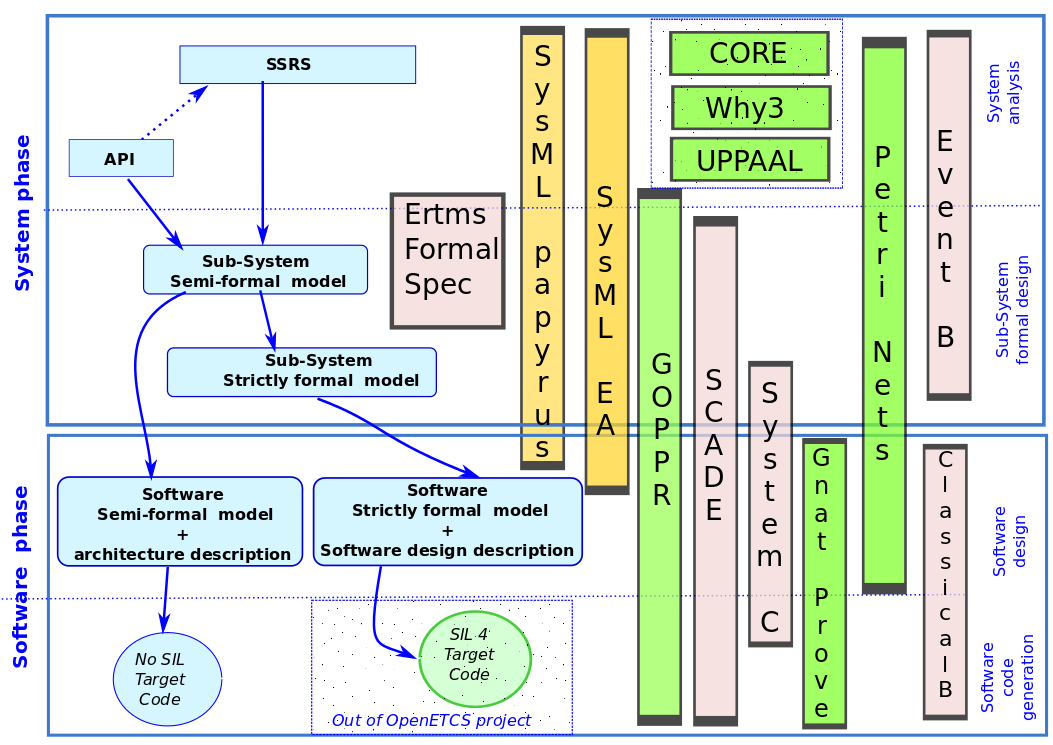
\includegraphics[width=\linewidth]{images/First.png}}
  \caption{Results of candidates}
  \label{fig:results}
\end{figure}

\subsection{Assessment}
\label{sec:assessment}

Each Benchmark was assessed by its author and by two additional assessors (in the case of Petri Nets and GNATprove, there was just one assessor).  This has been documented in \citep{WP7_O719}, which contains the ``raw data'', as well as some rudimentary aggregation of the data and some analysis.

The criteria in \citep{WP7_O719} were derived from WP2 requirements and quantified on scale from 0 to 3.  The results were recorded as the sum of the author and the two assessors, resulting in a score from 0 to 9 for each criteria.  The benchmarks with only one assessor have been adjusted by interpolating the score, shown in parentheses.

To give an idea of the results, Table~\ref{tab:phaseresults} shows the aggregated result of the benchmark for process phases.  These results must be taken with a grain of salt: This aggregation simply averages all relevant scores, thereby giving all criteria equal weight.  This is an unrealistic (and dangerous) assumption.  In fact, in the case of the criteria ``open source'' it created a real problem.  As Open Proof is the foundation of openETCS, using a closed-source tool with no open alternative should be a show stopper.  But this does not appear in the results of \citep{WP7_O719}.

Further, not all criteria could be quantified easily, resulting in surprising and suspicious results.  For instance, the assessments of Papyrus and Enterprise Architect sometimes differed drastically, even in areas where the notation (and not the tool) was concerned.  This was not expected, as both tools support the same notation.  This means that the results must be inspected carefully, before drawing conclusions.

 \begin{table}
  \centering
\begin{tabular}{|l | c | c | c | c | c | c | c | c | c | c |}
\hline
&  \rotatebox{90}{GOPRR} & \rotatebox{90}{ERTMSFormalSpecs} &  \rotatebox{90}{SysML with Papyrus} &  \rotatebox{90}{SysML with EA} &  \rotatebox{90}{SCADE} &  \rotatebox{90}{Event-B} &  \rotatebox{90}{Classical B} &  \rotatebox{90}{System C} & \rotatebox{90}{Petri Nets} &  \rotatebox{90}{GNATprove} \\
\hline 
System Analysis & \textcolor{blue}{5} & 1     & \textcolor{magenta}{7} & \textcolor{red}{\textbf{9}} & 3     & \textcolor{red}{\textbf{9}} & 3     & 2 & \textcolor{red}{\textbf{6(9)}}  & 2 (3) \\
\hline
Sub-system formal design  & \textcolor{red}{\textbf{9}} & \textcolor{red}{\textbf{9}} & \textcolor{blue}{6} & \textcolor{magenta}{7} & \textcolor{red}{\textbf{9}} & \textcolor{red}{\textbf{9}} & \textcolor{blue}{5} & \textcolor{blue}{5}  & \textcolor{red}{\textbf{6(9)}}   & 3 (4) \\
\hline
Software design  & \textcolor{red}{\textbf{9}} & \textcolor{green}{0} & \textcolor{blue}{6} & \textcolor{magenta}{7} & \textcolor{red}{\textbf{9}} & \textcolor{blue}{6} & \textcolor{red}{\textbf{9}} & \textcolor{red}{\textbf{9}} & \textcolor{red}{\textbf{6(9)}}   & \textcolor{red}{\textbf{6(9)}}  \\
\hline
Software code generation  & \textcolor{red}{\textbf{9}} & \textcolor{green}{0} & 3     & 3     & \textcolor{red}{\textbf{9}} & 3     & \textcolor{red}{\textbf{9}} & \textcolor{blue}{6} & 2 (3) & \textcolor{red}{\textbf{6(9)}}   \\
\hline
\end{tabular}
  \caption{Use of the approaches during process phases}
  \label{tab:phaseresults}
\end{table}

\subsection{Decision Meeting}
\label{sec:decision_meeting}

On July 4th, a WP7 workshop took place with the objective of choosing suitable tools for the toolchain.  To ease the process, the results from \citep{WP7_O719} were condensed into Figure~\ref{fig:results}.  The vertical stripes represent the individual tools.  The length and position of the stripe is determined by Table~\ref{tab:phaseresults}. The bar only covers area with a score of 6 or higher.

\subsubsection{SysML}

Using the available data as the foundation, the objective was to narrow the choices down as much as possible.  One obvious redundancy was the availability of two SysML tools, Papyrus and Enterprise Architect. After discussion of pros and cons of each, the partners agreed that Papyrus covers better the objectives of the project, especially the open-source requirement. 

Further, by vote, all the partners agree on the use Papyrus/SysML to cover the highest level of the  OpenETCS V-cycle.

\subsubsection{Short List}

Due to the evaluation and discussion during the decision meeting, the partners agreed on a short-list of six approaches. These are shown in red in Figure~\ref{fig:short}. and include the following:

\begin{tabular}{ p{0.5\linewidth} p{0.5\linewidth} }
SCADE & ERTMSFormalSpecs \\
SysML with Papyrus & System C \\
Classical B with Atelier B & Event-B with Rodin
\end{tabular}


 \begin{figure}
  \centering
  \fbox{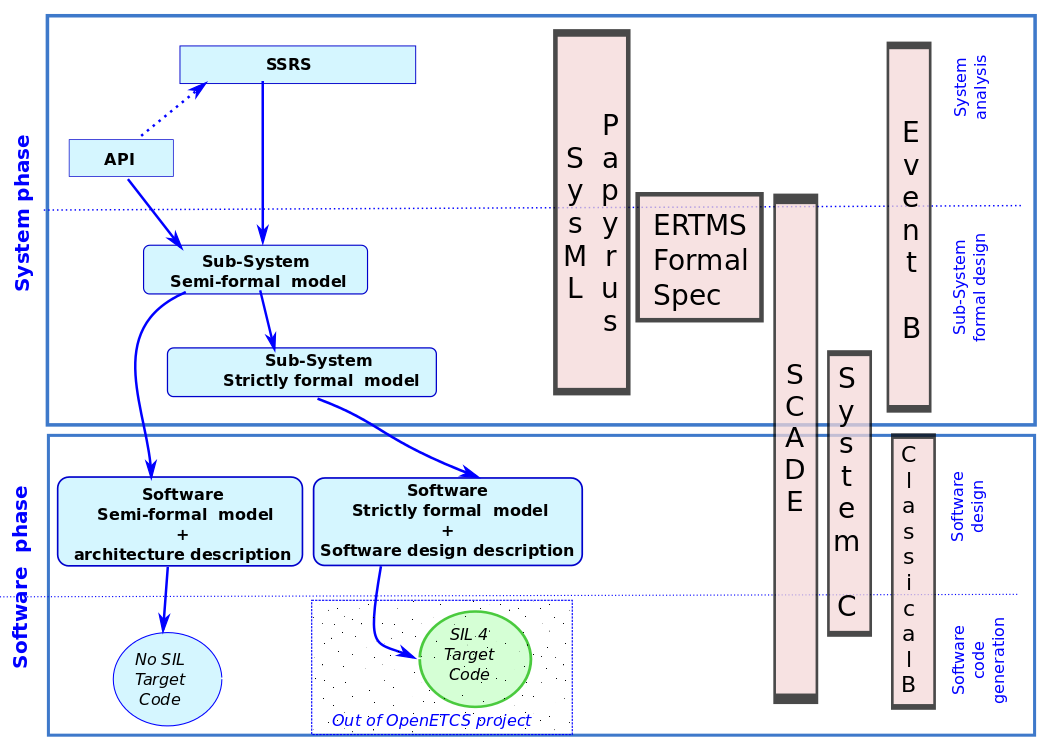
\includegraphics[width=\linewidth]{images/Short.png}}
  \caption{Short list}
  \label{fig:short}
\end{figure}

\subsection{Composition of Toolchains}
\label{sec:composition_of_tool_chains}

One toolchain was already suggested during the Paris meeting, namely Papyrus and SCADE.  Nevertheless, partners had the chance to propose additional toolchains using the tools from the shortlist.  It was necessary to find alternatives, as one severe weakness of the Papyrus/SCADE solution had already been pointed out in Paris: By not being open source, this solution would miss one of the main objectives of openETCS.

Two more toolchains have been proposed, resulting in three toolchains in total.  These have been documented by their respective owners in the appendices.

\subsection{Documenting the Decision}
\label{sec:documenting_the_decision}

What has been documented so far is a promising foundation for an openETCS primary toolchain.  However, it is not clear on how to proceed from here, as there are multiple competing avenues.  Resources in the project are thin and should be employed wisely.  Therefore, Section~\ref{sec:decision} contains an elaborate analysis with clear decisions that will guide the activities of the next six month, ensuring that we will choose the best option for openETCS while minimizing risk.



